\section{Lepton Universality in the Standard Modell}
\frame{\tableofcontents[currentsection]}
\begin{frame}{Standard Model (SM)}
    \begin{columns}
        \begin{column}{0.5\textwidth}
          \begin{itemize}
            \item gauge theory
            \item $SU(3)_C \otimes SU(2)_L \otimes U(1)_y $ \visible<4>{ $\overset{SSB}{\rightarrow} SU(3)_C \otimes U(1)_\text{QED}$}
            \only<2, 3>{
            \begin{itemize}
                \item strong interaction
                \item EM interaction
                \item weak interaction
            \end{itemize}}
            \only<4>{
              \begin{itemize}
                \item Masses generated
                \item Higgs-Boson
              \end{itemize}
            }
            \visible<3, 4>{
            \item twelve elementary fermions
            \begin{itemize}
                \item six quarks
                \item six leptons
                \item three generations
            \end{itemize}}
          \end{itemize}
        \end{column}
        \begin{column}{0.5\textwidth}
          \begin{figure}
            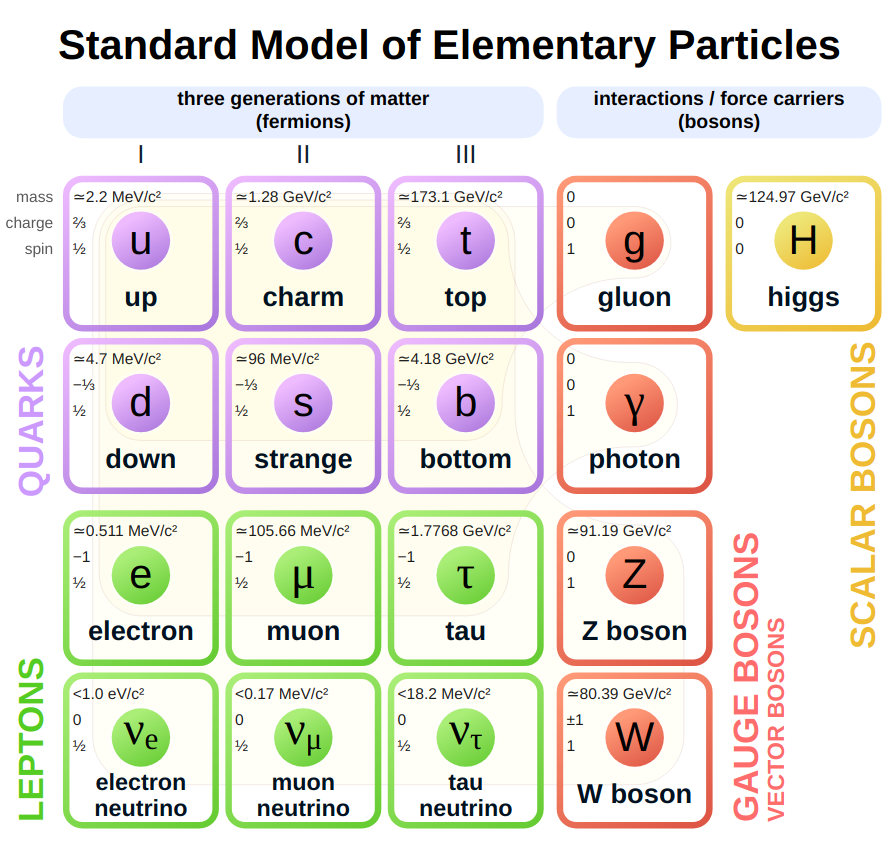
\includegraphics[width=0.8\textwidth]{content/images/SM.png}
            \caption*{Standard Model of particle physics \footnotemark{} }
          \end{figure}
        \end{column}
      \end{columns}
      \setcounter{footnote}{0}
      \stepcounter{footnote}{ \footnotetext{\url{https://en.wikipedia.org/wiki/Standard_Model}}}
\end{frame}

%\begin{frame}{Standard Model (SM)}
%  \begin{columns}
%    \begin{column}{0.5\textwidth}
%      \begin{itemize}
%        \item Spontaneous Symmetry Breaking
%        \begin{itemize}
%          \item $SU(3)_C \otimes SU(2)_L \otimes U(1)_\gamma \overset{SSB}{\rightarrow} SU(3)_C \otimes U(1)_\text{QED}$
%          \item Masses generated
%          \item Higgs-Boson
%        \end{itemize}
%      \end{itemize}
%    \end{column}
%    \begin{column}{0.5\textwidth}
%      \begin{figure}
%        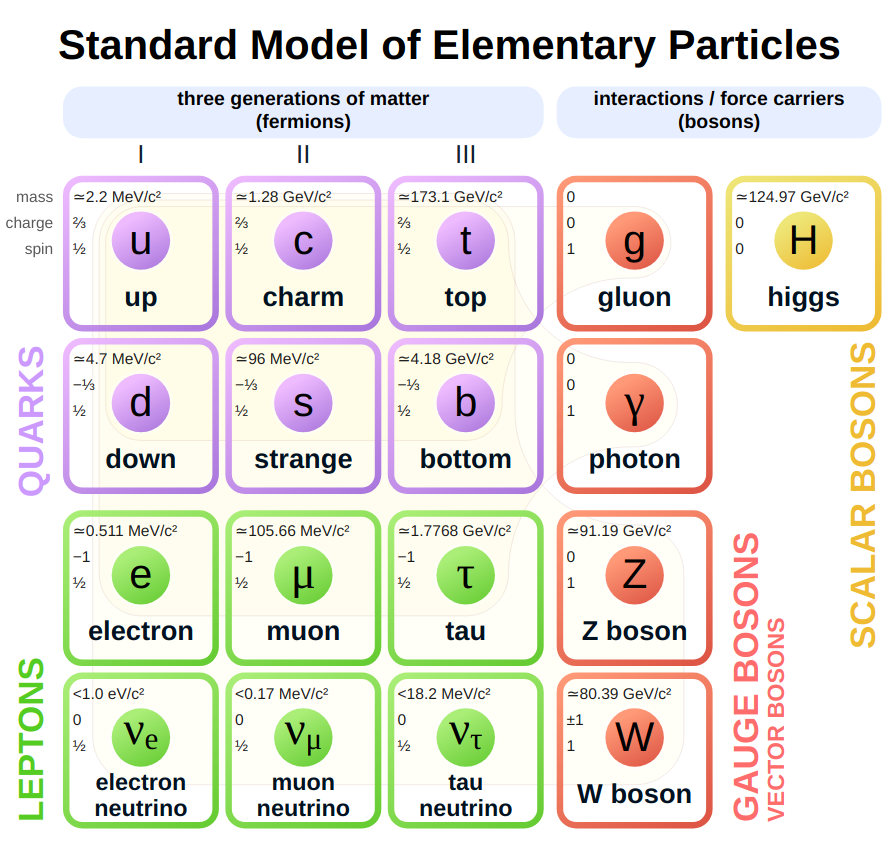
\includegraphics[width=0.8\textwidth]{content/images/SM.png}
%        \caption*{Standard Model of particle physics \footnotemark}
%      \end{figure}
%    \end{column}
%  \end{columns}
%  \footnotetext[1]{\url{https://en.wikipedia.org/wiki/Standard_Model}}
%\end{frame}

\begin{frame}{Leptons in the Standard Model}
  \begin{table}[]
    \begin{tabular}{lllll}
    \toprule 
    \textbf{Particle} & {\textbf{Q}$\:/\: \mathrm{e}$} & {\textbf{Mass}$\:/\: \mathrm{MeV}$} \\ 
    \midrule
     electron ($e$) & -1 &  0.511  \\
     neutrino ($\nu_e$) & 0 &  0  \\
     \midrule
     muon ($\mu$) & -1 &  105.66  \\
     neutrino ($\nu_\mu$) & 0 & 0 \\
     \midrule
     tau ($\tau$) & -1 & 1776.86 \\
     neutrino ($\nu_\tau$) & 0 & 0 \\
     \bottomrule
    \end{tabular}
\end{table}
\end{frame}

